\chapter{Coloring}

\section{Vertex coloring}

\begin{definition}[Coloring]
    A \vocab{(proper) coloring} of a graph \(G\)
    is a function \(c \colon V(G) \to \{1, 2, 3, \ldots\}\)
    such that \(c(u) \neq c(v)\) for every edge \(uv \in E(G)\).
\end{definition}

Note that a coloring of \(G\) is the same as a partition of \(V(G)\) into independent sets; that is, the induced subgraph on the vertices of each color is an independent set.

\begin{definition}[Chromatic Number]
    The \vocab{chromatic number} of a graph \(G\), denoted \(\chi(G)\), is the smallest \(k\) such that \(G\) has a \(k\)-coloring.
\end{definition}

\begin{proposition}
    For a planar graph \(G\),
    the chromatic number of \(G\)
    equals the flow number of its planar dual \(G^*\).
\end{proposition}

\begin{proof}[Sketch]
    Let \(G\) be a planar graph.
    Let \(c \colon V(G) \to \{1, 2, \ldots, k\}\) be a \(k\)-coloring of \(G\).

    Let \(R, S\) be adjacent regions in the plane embedding of \(G\), and let \(e = uv\) an the edge of \(G\) separating \(R\) and \(S\).
    Assume that \(u\) and \(v\) are adjacent in the clockwise order around \(R\).
    Hence, \(u\) and \(v\) are adjacent in the counterclockwise order around \(S\).
    We assign the flow \(f(e, R, S) = c(u) - c(v)\).

    It is straightforward to check that this is a \(k\)-flow.

    The converse is possible as well.
\end{proof}

For any graph \(G\) and for any order \(v_1, v_2, \ldots, v_n\) of \(V(G)\), we can define the \vocab{greedy coloring} of \(G\) with respect to this order by giving each vertex \(v_i\) the smallest color not used by its neighbors \(v_j\) with \(j < i\).
This coloring uses at most \(\Delta(G) + 1\) colors,
where \(\Delta(G)\) is the maximum degree of \(G\).

Let \(\delta(G)\) be the minimum degree of \(G\).

\begin{lemma} \label{lem:greedy-coloring-any-order}
    Let \(G\) be a graph and let \(v_1, v_2, \ldots, v_n\) be an order of \(V(G)\).
    Let \(t_i\) be the degree of \(v_i\) in the subgraph induced by \(v_1, v_2, \ldots, v_i\).
    Then the greedy coloring of \(G\) with respect to this order uses at most \(\max_i t_i + 1\) colors.
\end{lemma}

\begin{proof}
    At the \(i\)\textsuperscript{th} step,
    the vertex \(v_i\) is colored with the smallest color not used by its neighbors \(v_j\) with \(j < i\).
    Since there are \(t_i\) of such neighbors,
    the color of \(v_i\) is at most \(t_i + 1\).

    Hence, for all \(i\),
    the color of \(v_i\) is at most \(\max_i t_i + 1\),
    and the lemma follows.
\end{proof}

\begin{theorem} \label{thm:greedy-coloring-induced-subgraph}
    Let \(G\) be a graph and let
    \begin{equation}
        k = \max_{H \subseteq G} \delta(H),
    \end{equation}
    where the maximum is taken over all induced subgraphs \(H\) of \(G\).
    Then \(\chi(G) \leq k + 1\).
\end{theorem}

\begin{proof}
    Assume that \(x_n, x_{n - 1}, \ldots, x_{i+1}\) have been defined.
    Let \(x_i\) be the vertex of minimum degree in the subgraph induced by \(V(G) \setminus \{x_{i + 1}, x_{i + 2}, \ldots, x_n\}\).
    Let \(t_i\) be the degree of \(x_i\) in the subgraph induced by \(\{x_1, x_2, \ldots, x_i\} = V(G) \setminus \{x_{i + 1}, x_{i + 2}, \ldots, x_n\}\).
    Note that \(t_i = \delta(G[\{x_1, x_2, \ldots, x_i\}]) \leq k\).
    Hence, by Lemma~\ref{lem:greedy-coloring-any-order},
    the greedy coloring of \(G\) with respect to the order \(x_1, x_2, \ldots, x_n\) uses at most \(k + 1\) colors.
\end{proof}

\begin{corollary} \label{cor:greedy-coloring-delta-plus-one}
    Let \(G\) be a graph.
    Then \(\chi(G) \leq \Delta(G) + 1\).
\end{corollary}

Recall that a graph that is connected but not \(2\)-connected has a block decomposition: a tree-like structure consisting of maximal connected subgraphs without a cut vertex, that intersect only at cut vertices.

\begin{proposition}
    If \(G = K_n\), then \(\chi(G) = n = \Delta(G) + 1\).
\end{proposition}

\begin{proposition}
    If \(G = C_{2n + 1}\), then \(\chi(G) = 3 = \Delta(G) + 1\).
\end{proposition}

\begin{theorem}[Brooks' Theorem] \label{thm:brooks-theorem}
    Let \(G\) be a connected graph that is not a complete graph or an odd cycle.
    Then \(\chi(G) \leq \Delta(G)\).
\end{theorem}

\begin{proof}
    Assume, by induction, that the theorem holds for all graphs with fewer vertices than \(G\).

    We solve \(\Delta(G) \leq 2\) separately.

    Suppose that \(G\) has a vertex \(x_n\) of degree less than \(\Delta(G)\).
    If \(H\) is an induced graph of \(G\) that contains \(x_n\),
    then \(\delta(H) \leq \deg(x_n) \leq \Delta(G) - 1\).
    If \(H\) is an induced graph of \(G\) that does not contain \(x_n\),
    then there exists an edge \(e = vu\) where \(v \in V(H)\) and \(u \in V(G) \setminus V(H)\).
    Then, \(\delta(H) \leq \deg_H(v) \leq \deg_G(v) - 1 \leq \Delta(G) - 1\).
    Therefore, by Lemma~\ref{lem:greedy-coloring-any-order},
    \(\chi(G) \leq \Delta(G)\).
    Thus, we assume that \(G\) is \(\Delta(G)\)-regular.

    Suppose that \(G\) has a cut-vertex \(v\); that is, there exists sets \(A\) and \(B\) such that \(A \cup B = V(G)\), \(A \cap B = \{v\}\), no edge connects \(A \setminus \{v\}\) and \(B \setminus \{v\}\).
    Therefore, \(E(G) = E(G[A]) \cup E(G[B])\).

    We claim that \(G\) contains vertices \(x_1, x_2, x_n\) such that \(x_1x_2 \notin E(G)\), \(x_1x_n \in E(G)\), \(x_2x_n \in E(G)\), and \(G - \{x_1, x_2\}\) is connected.
    \begin{proof}
        Suppose \(G\) is \(3\)-connected
        Since \(G\) is not the complete graph,
        there exists \(u, v \in V(G)\) such that \(uv \notin E(G)\).
        Since \(G\) is connected, there exists a path \(u = u_1, u_2, \ldots, u_\ell = v\) in \(G\), where \(\ell \geq 3\).
        Define
        \begin{equation}
            x_1 = u_1, x_n = u_2, x_2 = u_3.
        \end{equation}
        Note that \(3\)-connectivity guarantees that \(G - \{x_1, x_2\}\) is connected.

        Otherwise, suppose that \(G\) is not \(3\)-connected.
        Hence, there exists a vertex \(x_n\) such that \(G - \{x_n\}\) is not \(2\)-connected.
        We know that \(G - \{x_n\}\) is connected since \(G\) is \(2\)-connected.

        Then, \(G - \{x_n\}\) has a block decomposition, and it has two blocks \(B_1\) and \(B_2\) that contain only one cut vertex of \(G - \{x_n\}\), respectively denoted by \(v_1\) and \(v_2\).

        Since \(G\) is \(2\)-connected, the \(v_i\) is not a cut vertex of \(G\) for \(i \in \{1, 2\}\).
        Therefore, \(x_n\) is adjacent to some vertex \(x_i\) in \(B_i \setminus \{v_i\}\) for \(i \in \{1, 2\}\).
        Since \(x_1, x_2\) are in different blocks, \(x_1x_2 \notin E(G)\).
        Moreover, \(G - \{x_1, x_2\}\) is connected since \(\deg(x_n) \geq 3\).
    \end{proof}

    Let \(x_1, x_2, x_n\) be as in the claim.
    For \(i \in \{n-1, n-2, \ldots, 3\}\),
    assume \(x_{i+1}, x_{i+2}, \ldots, x_n\) have been defined.
    We define \(x_i\) to be a neighbor of some \(x_{i+1}\), \(x_{i+2}\), \(\ldots\), \(x_n\) in \(G - \{x_1, x_2\}\), which exists since \(G - \{x_1, x_2\}\) is connected.

    Let \(c \colon V(G) \to \mathbb{Z}\) be a the greedy coloring of \(G\) with respect to the order \(x_1, x_2, \ldots, x_n\).
    Since \(x_1x_2 \notin E(G)\), \(c(x_1) = c(x_2) = 1\).
    For each \(i \in \{3, 4, \ldots, n-1\}\),
    \(x_i\) has at most \(\Delta(G) - 1\) neighbors in \(\{x_1, x_2, \ldots, x_{i-1}\), and hence \(c(x_i) \leq \Delta(G)\).
    Moreover, since \(x_1\) and \(x_2\) are adjacent to \(x_n\) and \(c(x_1) = c(x_2)\), the \(\Delta(G)\) neighbors of \(x_n\) have at most \(\Delta(G) - 1\) colors, and hence \(c(x_n) \leq \Delta(G)\).
    Therefore, \(\chi(G) \leq \Delta(G)\), and the theorem follows.
\end{proof}

\begin{question}
    If \(G\) satisfies \(\chi(G) = \Delta(G)\),
    does \(G\) contain a copy of \(K_{\Delta(G)}\)?
\end{question}

The answer to this question in general is not known.

\begin{conjecture}[Borodin--Kostochka Conjecture]
    If \(G\) satisfies \(\chi(G) \geq \Delta(G) \geq 9\),
    then \(G\) contains a copy of \(K_{\Delta(G)}\).
\end{conjecture}

\begin{theorem}
    If \(G\) is a graph with \(\chi(G) = \Delta(G) = 13\),
    then \(G\) contains a copy of \(K_{\Delta - 3}\).
\end{theorem}

\begin{question}
    Does \(\chi(G) \geq k\) imply that \(G\) contains a large (in terms of \(k\)) complete graph?
\end{question}

The answer is no, and that's what will be shown next.

\begin{theorem}
    Let \(k \geq 1\) be an integer.
    There exists a triangle-free graph \(G_k\) with \(\chi(G_k) = k\).
\end{theorem}

\begin{proof}[Proof (Mycielski's Construction)]
    Let \(G_1\) be the graph with one vertex and no edges,
    let \(G_2 = K_2\), and let \(G_{3} = C_5\).

    Let \(k \geq 4\) and \(G_{k-1}\) be a triangle-free graph with \(\chi(G_{k-1}) = k-1\) with
    \begin{equation}
        V(G_{k-1}) = \{v_1, v_2, \ldots, v_n\}.
    \end{equation}

    Let \(G_k\) be the graph with vertex set
    \begin{equation}
        V(G_k) = \{v_1, v_2, \ldots, v_n, u_1, u_2, \ldots, u_n, x\},
    \end{equation}
    and edge set
    \begin{equation}
        \thickmuskip=10mu
        \medmuskip=10mu
        E(G_k)
        = E(G_{k-1})
        \cup \big\{v_iu_j : v_iv_j \in E(G_{k-1})\big\}
        \cup \big\{xu_i : 1 \leq i \leq n\big\}.
    \end{equation}

    Assume, by the sake of contradiction, that \(T \subset V(G_k)\) induces a triangle in \(G_k\).
    Since the neighborhood of \(x\) is \(\{u_1, u_2, \ldots, u_n\}\) which is independent, \(x \notin T\).
    Since \(\{u_1, u_2, \ldots, u_n\}\) is independent, \(T \cap \{u_1, u_2, \ldots, u_n\} \leq 1\).
    Therefore, \(T = \{v_i, v_j, w_k\}\), where \(w_k \in \{u_k, v_k\}\).
    This implies that \(T' = \{v_i, v_j, v_k\}\) induces a triangle in \(G_{k-1}\), which is a contradiction.
    Therefore, \(G_k\) is triangle-free.

    Let \(c \colon V(G_{k-1}) \to \{1, 2, \ldots, k-1\}\) be a coloring of \(G_{k-1}\) with \(\chi(G_{k-1}) = k-1\).
    Then, let \(\tilde{c} \colon V(G_k) \to \{1, 2, \ldots, k\}\)
    be defined by
    \begin{equation}
        \tilde{c}(v_i) = \tilde{c}(u_i) = c(v_i),
        \quad
        \tilde{c}(x) = k.
    \end{equation}
    It is straightforward to check that \(\tilde{c}\) is a proper coloring of \(G_k\), and hence \(\chi(G_k) \leq k\).

    Assume, by the sake of contradiction, that
    \(c \colon V(G_k) \to \{1, 2, \ldots, k-1\}\)
    is a proper coloring of \(G_k\).
    Assume that \(c(x) = k-1\).
    Hence, \(c(u_i) \neq k-1\) for all \(i\).
    Define \(\tilde{c} \colon V(G_{k-1}) \to \{1, 2, \ldots, k-2\}\) by
    \begin{equation}
        \tilde{c}(v_i) =
        \begin{cases}
            c(v_i) & \text{if } c(v_i) \neq k-1, \\
            c(u_i) & \text{if } c(v_i) = k-1.
        \end{cases}
    \end{equation}
    Let \(v_i, v_j \in V(G_{k-1})\) be adjacent.
    Hence, \(c\) colors \(v_i\) and \(v_j\) with different colors, and hence at most one of them is colored with \(k-1\).
    If neither of them is colored with \(k-1\), then
    \begin{equation}
        \tilde{c}(v_i) = c(v_i) \neq c(v_j) = \tilde{c}(v_j).
    \end{equation}
    If one of them is colored with \(k-1\), say \(v_i\), then
    \begin{equation}
        \tilde{c}(v_i) = c(u_i) \neq c(v_j) = \tilde{c}(v_j),
    \end{equation}
    since \(u_i\) and \(v_j\) are adjacent in \(G_k\).
    Therefore, \(\tilde{c}\) is a proper \((k-2)\)-coloring of \(G_{k-1}\), which is a contradiction.
    Therefore, \(\chi(G_k) \geq k\).

    Finally, \(\chi(G_k) = k\), and the theorem follows.
\end{proof}

Let the \vocab{clique number} of a graph \(G\), denoted \(\omega(G)\), be the maximum size of a complete subgraph of \(G\).

\begin{conjecture}[Reed]
    For all graphs \(G\),
    \begin{equation}
        \chi(G) \leq \left\lceil \frac{\Delta(G)+1}{2} + \frac{\omega(G)}{2} \right\rceil.
    \end{equation}
\end{conjecture}

The graph with vertices \(v_{ij}\) for \(i \in \{1, 2, 3, 4, 5\}\) and \(j \in \{1, 2, \dots, n\}\) where \(v_{ij}\) is connected to \(v_{k\ell}\) if and only if \(i-k \equiv \pm 1 \pmod{5}\) shows that the conjecture is tight.

\begin{figure}[htbp]
    \centering
    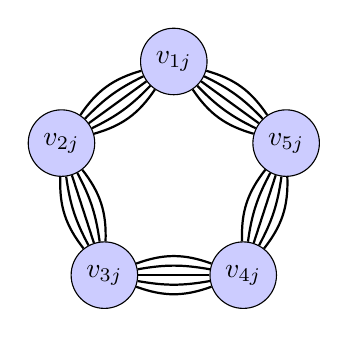
\begin{tikzpicture}[scale=1.5,
            blob/.style={circle, draw, minimum size=0.6cm, fill=blue!20},
            edge/.style={thick}
        ]

        % Define positions for the 5 blobs arranged in a pentagon
        \foreach \i [count=\n from 1] in {90, 162, 234, 306, 18} {
                \node[blob] (I\n) at (\i:1) {$v_{\n j}$};
            }

        % Connect each blob to its two neighbors with multiple edges
        \foreach \n in {1,...,5} {
                % Calculate the next and previous indices modulo 5
                \pgfmathtruncatemacro{\next}{mod(\n,5)+1}

                % Draw two parallel edges to represent multiple connections
                \foreach \angle in {-20, -10, ..., 20} {
                        \draw[edge] (I\n) to[bend left=\angle] (I\next);
                    }
            }
    \end{tikzpicture}
    \caption{The graph showing that Reed's Conjecture is tight.}
\end{figure}

Let \(n, k\) be positive integers, with \(k \leq n\).
The \vocab{Kneser graph} \(K(n, k)\) has vertices the \(k\)-element subsets of \(\{1, 2, \ldots, n\}\), where two vertices are adjacent if and only if the corresponding subsets are disjoint.

Note that \(K(n, 1) = K_n\).
If \(k > \frac{n}{2}\), then \(K(n, k)\) has no edges.
If \(k = \frac{n}{2}\), then \(K(n, k)\) is a matching.
Usually, we will focus on the case where \(k < \frac{n}{2}\).

\begin{figure}[htbp]
    \centering
    \begin{tikzpicture}[scale=.7]
        \tikzset{every node/.style={inner sep=2pt, minimum size=10pt}}
        \graph[math nodes, clockwise]
        { subgraph I_n [V={35,23,24,14,15}] --
        subgraph C_n [V={12,45,13,25,34},radius=1cm];
        {[cycle] 35,24,15,23,14} };
    \end{tikzpicture}
    \caption{The Kneser graph \(K(5, 2)\), isomorphic to the Petersen graph.}
\end{figure}

\begin{question}
    What is the chromatic number of \(K(n, k)\)?
\end{question}

\begin{lemma}
    \(\chi((K(2k+\ell, k))) \leq \ell+2\).
\end{lemma}

\begin{proof}
    For \(i \in \{1, 2, 3, \ldots, \ell+1\}\),
    color with color \(i\) the vertices corresponding to the \(k\)-element subsets whose smaller element is \(i\) --- which form an independent set.
    The remaining vertices are the \(k\)-element subsets of the \((2k-1)\)-element set \(\{\ell + 2, \ell + 3, \ldots, 2k + \ell\}\),
    and hence they form an independent set, which we color with color \(\ell + 2\).
\end{proof}

\begin{theorem}[Kneser's Conjecture] \label{thm:kneser-conjecture}
    Let \(k\) and \(\ell\) be positive integers.
    Then, \(\chi(K(2k+\ell), k) = \ell + 2\).
\end{theorem}

This was proven independently by Bárány (1978) and Lovász (1978).
We will present Lovász's proof, and we will use theorems from topology to prove this result.

The \(n\)-dimensional Euclidean space \(\mathbb{R}^n\)
is equipped with the usual inner product \(\langle x, y \rangle\),
norm \(\|x\| = \left( \langle x, x \rangle \right)^{\frac{1}{2}}\),
and distance \(d(x, y) = \|x - y\|\).
Recall that a set \(U \subset \mathbb{R}^n\) is \vocab{open}
if for all \(u \in U\), there exists \(\delta > 0\) such that
the ball \(B_\delta(u)\) of radius \(\delta\) centered at \(u\)
satisfies \(B_\delta(u) \subset U\).
Recall that \(f \colon \mathbb{R}^n \to \mathbb{R}\) is \vocab{continuous at \(x \in \mathbb{R}^n\)} if for all \(\varepsilon > 0\), there exists \(\delta > 0\) such that for all \(y \in \mathbb{R}^n\), if \(d(x, y) < \delta\), then \(\left| f(x) - f(y) \right| < \varepsilon\).
We say that \(f\) is \vocab{continuous} if it is continuous at all \(x \in \mathbb{R}^n\).

The \vocab{\(\ell\)-dimensional sphere \(S_\ell\)} is 
\begin{equation}
    S_\ell = \left\{ x \in \mathbb{R}^{\ell+1} : \|x\| = 1 \right\}.
\end{equation}
The \vocab{open hemisphere \(H(a)\)} centered at \(a \in S_\ell\) is
\begin{equation}
    H(a) = \left\{ x \in S_\ell : \langle x, a \rangle > 0 \right\}.
\end{equation}
Points \(x\) and \(-x\) in \(S_\ell\) are said to be \vocab{antipodal}.

We know that \(f \colon \mathbb{R}^n \to \mathbb{R}\) is continuous if and only if for all open sets \(U \subset \mathbb{R}\), the preimage \(f^{-1}(U)\) is open in \(\mathbb{R}^n\).
Moreover, we say that \(S \subset \mathbb{R}^n\), we say that \(U \subset S\) is \vocab{relatively open} if there exists an open set \(V \subset \mathbb{R}^n\) such that \(U = V \cap S\).
We also know that any union of open sets is open, and any finite intersection of open sets is open.

\begin{theorem}[Borsuk--Ulam Theorem] \label{thm:borsuk-ulam}
    Let \(f \colon S^\ell \to \mathbb{R}^\ell\) be continuous.
    Then there exists \(x \in S^\ell\) such that \(f(x) = f(-x)\).
\end{theorem}

\begin{theorem}[Lusternik--Schnirelmann Theorem] \label{thm:lusternik-schnirelmann}
    If \(A_1, \dots A_{\ell + 1} \subset S^\ell\) are relatively open sets such that \(S^\ell = A_1 \cup \dots \cup A_{\ell + 1}\),
    then there exists \(i\) such that \(A_i\) contains a pair of antipodal points.
\end{theorem}

\nameref{thm:borsuk-ulam} and \nameref{thm:lusternik-schnirelmann} are equivalent theorems, the former is the algebraic topology variant, and the latter is the set convering variant.
We do not prove these theorems here, and we use \nameref{thm:lusternik-schnirelmann} in the proof of \nameref{thm:kneser-conjecture}.

\begin{theorem}[Gale's Theorem] \label{thm:gale}
    Let \(k\) and \(\ell\) be positive integers.
    There exists a set of \(2k+\ell\) points in \(S_\ell\)
    such that every open hemishere contains at least \(k\) of them.
\end{theorem}

\begin{proof}
    Let \(v = 2k + \ell\) and \(m = k-1\).
    Let \(a_1, \dots a_v\) be any \(v\) distinct points real numbers,
    and define the \((2m+1) \times v\) matrix \(G\) (in the moment curve) by
    \begin{equation}
        G =
        \begin{bmatrix}
            1 & 1 & \cdots & 1 \\
            a_1 & a_2 & \cdots & a_v \\
            a_1^2 & a_2^2 & \cdots & a_v^2 \\
            \vdots & \vdots & \ddots & \vdots \\
            a_1^{2m} & a_2^{2m} & \cdots & a_v^{2m}
        \end{bmatrix}.
    \end{equation}

    Let \(r_0, r_1, \ldots, r_{2m}\) be the row vectors of \(G\).
    Suppose \(b_0, b_1, \ldots, b_{2m}\) are real numbers such that
    \begin{equation}
        \sum_{i=0}^{2m} b_i r_i = 0.
    \end{equation}
    Let \(f(x) = \sum_{i=0}^{2m} b_i x^i\).
    Then, \(a_1, a_2, \ldots, a_v\) are distinct roots of \(f\).
    Since \(\deg f = 2m < v\),
    \(f\) is the zero polynomial,
    and hence \(b_0 = b_1 = \cdots = b_{2m} = 0\).
    Therefore, the row vectors of \(G\) are linearly independent,
    and consequently \(\operatorname{rk}(G) = 2m+1\).

    Consider the null space \(W\) of \(G\), that is,
    \begin{equation}
        W = \left\{ w \in \mathbb{R}^v : Gw = 0 \right\}.
    \end{equation}
    By the rank-nullity theorem, we have
    \begin{equation}
        \dim W = v - \operatorname{rk}(G) = v - (2m+1) = \ell + 1.
    \end{equation}

    Consider a nonzero \(w = (w_1, \ldots, w_v) \in W\).
    Assume, by the sake of contradiction,
    that \(w\) has at most \(m\) negative entries.
    Define the polynomial
    \begin{equation}
        g(x) = \prod_{i : w_i < 0} (x - a_i)
    \end{equation}
    with degree at most \(m\).
    Then, \(g(x)^2\) is a polynomial of degree at most \(2m\)
    which vanishes at \(a_1, a_2, \ldots, a_v\) and otherwise is positive.
    Let \(b_0, b_1, \ldots, b_{2m}\) be the coefficients of \(g(x)^2\), that is,
    \begin{equation}
        g(x)^2 = \sum_{i=0}^{2m} b_i x^i.
    \end{equation}
    Let \(b\) be the \((2m+1)\)-row vector with entries \(b_0, b_1, \ldots, b_{2m}\).
    Let \(y = \sum_{i=0}^{2m} b_i r_i = bG\) which is in the row-space of \(G\).
    Moreover, the \(i\)\textsuperscript{th} entry of \(y\) is non-negative for each \(i\), and it is zero if and only if \(w_i < 0\).
    On one hand, \(\langle y^T, w \rangle = bGw = 0\).
    On another hand, using that \(y_i = 0\) whenever \(w_i < 0\), we have
    \begin{equation}
        0 =
        \langle y^T, w \rangle =
        \sum_{i=1}^{v} y_i w_i =
        \sum_{i : w_i \geq 0} \underbrace{y_iw_i}_{> 0}
    \end{equation}
    which implies that \(w\) has no positive entries.
    However, since \(Gw = 0\), it follows that the sum of the entries of \(w\), \(r_1w\), is zero, and therefore \(w\) has no negative entries, which is a contradiction.

    Therefore, each nonzero vector \(w \in W\) has at least \(m+1 = k\) negative entries. Since \(-w \in W\) as well, each nonzero vector \(w \in W\) has at least \(m+1 = k\) positive entries.

    Let \(N\) be the \(v \times (v - 2m - 1)\) matrix whose columns form a basis for \(W\).
    Let \(z_1,\ldots, z_{v-2m-1}\) be the row vectors of \(N\).
    Let \(\bar{z}_i = z_i / \|z_i\|\) for \(i \in \{1, 2, \ldots, v-2m-1\}\).
    Let \(u \in \mathbb{R}^{\ell + 1}\) be nonzero.
    Then, \(Nu\) is a linear combination of the columns of \(N\),
    hence is in \(W\).
    So \(Nu\) has at least \(k\) negative entries and at least \(k\) positive entries.
    The \(i\)\textsubscript{th} entry of \(Nu\) is \(\langle z_i, u \rangle\),
    Hence, for any \(u\), at least \(k\) of the \(z_i\) satisfy \(\langle z_i, u \rangle < 0\).
    consequently, for any \(u \in S_\ell\), at least \(k\) of the \(\bar{z}_i\) satisfy \(\langle \bar{z}_i, u \rangle < 0\), as desired.
\end{proof}

We are now ready to prove Kneser's Conjecture.

\begin{proof}[Proof of \nameref{thm:kneser-conjecture}]
    We already know that \(\chi(K(2k+\ell, k)) \leq \ell + 2\).
    It suffices to show that \(\chi(K(2k+\ell, k)) > \ell + 1\).

    We will show that for any partition 
    \(C_1, \dots, C_{\ell+1}\)
    of the \(k\)-subsets of \(\{1, 2, \ldots, 2k+\ell\}\),
    some \(C_i\) contains two disjoint \(k\)-subsets.
    First, we identify \([2k+\ell]\) with the set \(V \subset S_\ell\) of points
    given by \nameref{thm:gale}.
    For \(i \in \{1, 2, \ldots, \ell+1\}\), let
    \begin{equation}
        A_i = \{
            a \in S_\ell :
            \text{the open hemisphere \(H(a)\) contains a \(k\)-subset of \(V\) in \(C_i\)}
        \}.
    \end{equation}
    By \nameref{thm:gale},
    \(S_\ell = A_1 \cup \dots \cup A_{\ell+1}\).
    We claim that each \(A_i\) is relatively open.
    First, note that for any \(a \in S_\ell\),
    the open hemisphere \(H(a)\) is open in \(S_\ell\)
    since it is the intersection of \(S_\ell\) and
    the preimage of \((0, \infty)\)
    under the continuous function \(x \mapsto \langle x, a \rangle\).

    Moreover, note that \(b \in H(a) \iff a \in H(b)\), and hence
    \begin{equation}
        A_i = \bigcup_{B \in C_i} \bigcap_{v \in C} H(v),
    \end{equation}
    that is, \(A_i\) is the union over all \(k\)-subsets \(B\) in \(C_i\) of the intersection of the open hemispheres centered at the points in \(B\).
    Since each open hemisphere is open in \(S_\ell\), and \(A_i\) is a union of finitely many intersections of open sets, \(A_i\) is relatively open in \(S_\ell\).

    By \nameref{thm:lusternik-schnirelmann},
    there exists \(i\) such that \(A_i\) contains a pair of antipodal points.
    Let \(a, -a\) be antipodal points in \(A_i\).
    Then, the open hemisphere \(H(a)\) contains a \(k\)-subset \(B_1\) of \(V\) in \(C_i\),
    and the open hemisphere \(H(-a)\) contains a \(k\)-subset \(B_2\) of \(V\) in \(C_i\).
    Since \(H(a) \cap H(-a) = \emptyset\),
    it follows that \(B_1 \cap B_2 = \emptyset\),
    and so \(C_i\) contains two disjoint \(k\)-subsets,
    that is, \(C_i\) is not an independent set in \(K(2k+\ell, k)\).

    Therefore,
    any partition of the vertices of \(K(2k+\ell, k)\) into \(\ell+1\) sets 
    has a set that is not an independent set,
    and hence \(\chi(K(2k+\ell, k)) > \ell + 1\).
\end{proof}

\section{Edge coloring}

\begin{definition}[Edge Coloring]
    Let \(G\) be a graph.
    An \vocab{edge coloring} of \(G\) is a function
    \(
        c \colon E(G) \to \{1, 2, \ldots\}
    \)
    such that if \(e_1\) and \(e_2\) are adjacent edges,
    then \(c(e_1) \neq c(e_2\).
    The \vocab{chromatic index} of \(G\),
    denoted \(\chi'(G)\),
    is the minimum \(k\) such that \(G\) has an edge coloring with \(k\) colors.
\end{definition}

\begin{definition}[Line graph]
    The \vocab{line graph} of a graph \(G\), denoted \(L(G)\), is the graph whose vertices are the edges of \(G\), and two vertices are adjacent if the corresponding edges are incident to a common vertex in \(G\).
\end{definition}

Note that \(\chi'(G) = \chi(L(G))\).

\begin{proposition} \label{prop:easy-bounds-edge-coloring}
    Let \(G\) be a graph.
    Then,
    \begin{equation}
        \Delta(G) \leq \chi'(G) \leq 2\Delta(G) - 1.
    \end{equation}
\end{proposition}

\begin{proof}[Proof of the lower bound]
    Let \(c \colon E(G) \to \{1, 2, \ldots, k\}\) be an edge coloring of \(G\).
    Let \(v\) be a vertex with \(\deg(v) = \Delta(G)\).
    The \(\Delta(G)\) edges incident to \(v\) have \(\Delta(G)\) distinct colors,
    and hence \(k \geq \Delta(G)\).
    Therefore, \(\chi'(G) \geq \Delta(G)\).
\end{proof}

\begin{proof}[Proof of the upper bound]
    Let \(G^*\) be the graph with vertex set \(E(G)\),
    where two vertices are adjacent if and only if the corresponding edges are incident to a common vertex.
    Let \(e \in E(G)\) be an edge.
    Let \(x\) and \(y\) be the vertices incident to \(e\).
    Then, the degree of \(e\) in \(G^*\) is \(\deg(x) + \deg(y) - 2 \leq 2\Delta(G) - 2\).
    Therefore, \(\Delta(G^*) \leq 2\Delta(G) - 2\),
    and consequently \(\chi'(G) \leq 2\Delta(G) - 1\) by Corollary~\ref{cor:greedy-coloring-delta-plus-one}.
\end{proof}

\begin{theorem}[Vizing's Theorem] \label{thm:vizing}
    Let \(G\) be a graph.
    Then,
    \begin{equation}
        \chi'(G) \leq \Delta(G) + 1.
    \end{equation}
\end{theorem}

We prove \nameref{thm:vizing} twice.
First, we prove it as done in the course, which can be watched in \href{https://youtu.be/9t76UcdgiGI}{Luke Postle's YouTube video}.
Second, we follow \href{https://homepages.cwi.nl/~lex/files/vizing.pdf}{Lex Schrijver's proof}.

What follows is the proof as done in the course.

\begin{definition}[Kempe Chain]
    Let \(\phi\) be a partial \(k\)-edge-coloring of a graph \(G\).
    If \(a, b \in [k]\) and \(v \in V(G)\),
    then the \vocab{\((a, b)\)-chain at \(v\)},
    denoted \(P_v(a, b, \phi)\),
    is the maximal path/cycle of \(a\)- and \(b\)-colored edges containing \(v\).
\end{definition}

\begin{definition}[Switching]
    The coloring \(\phi'\) obtained from \(\phi\) by \vocab{switching} the colors of the edges in \(P_v(a, b, \phi)\) is given by
    \begin{itemize}
        \item \(\phi'(e) = \phi(e)\) if \(e \notin P_v(a, b, \phi)\),
        \item \(\phi'(e) = \{a, b\} \setminus \phi(e)\) if \(e \in P_v(a, b, \phi)\).
    \end{itemize}
\end{definition}

\begin{definition}
    Let \(\phi\) be a partial \(k\)-edge-coloring of a graph \(G\).
    A color \(a \in [k]\) is \vocab{missing at \(v\)} if there is no edge incident to \(v\) colored with \(a\).
    We lt \(\phi(v)\) denote the set of colors missing at \(v\).
\end{definition}

\begin{definition}[Vizing fan]
    Let \(G\) be a graph,
    let \(e = v_0v_1\) be an edge of \(G\),
    and let \(\phi\) be a \(k\)-edge-coloring of \(G - e\).

    We say that \(T = (v_0e_1v_1e_2v_2 \cdots e_nv_n)\) is a \vocab{Vizing fan} with respect to \(e\), vertex \(v_0\), and coloring \(\phi\), If
    \begin{itemize}
        \item \(v_0, v_1, \ldots, v_n\) are distinct,
        \item \(e_j = v_0v_j\) for all \(1 \leq j \leq n\),
        \item \(\phi(e_j) \in \bigcup_{i < j} \phi(v_i)\) for all \(2 \leq j \leq n\).
    \end{itemize}
\end{definition}

\begin{lemma} \label{lem:vizing-fan-disjoint-colors}
    Let \(G\) be a graph, and \(e = v_0v_1 \in E(G)\).
    Assume that for some integer \(k \geq \Delta(G) + 1\),
    \(G - e\) has a \(k\)-edge-coloring, but \(G\) does not.
    If \(\phi\) is a \(k\)-edge-coloring of \(G - e\),
    and \(T = (v_0e_1v_1e_2v_2 \cdots e_nv_n)\) is a Vizing fan
    with respect to \(e\), vertex \(v_0\), and coloring \(\phi\),
    then
    \begin{equation}
        \phi(v_i) \cap \phi(v_j) = \emptyset,
    \end{equation}
    for all distict \(i, j \in \{0, 1, \ldots, n\}\).
\end{lemma}

\begin{proof}
    Assume by contradiction that there exists \(i < j \in [n]\) such that \(\phi(v_i) \cap \phi(v_j) \neq \emptyset\).
    Let \(\phi, T, i, j\) be chosen such that such that
    \(j\) is minimized, and subject to that,
    \(i\) is minimized.
    Let \(\alpha \in \phi(v_i) \cap \phi(v_j)\).

    One of the following three cases must hold:
    \(i = 0\) and \(j = 1\);
    \(i = 0\) and \(j > 1\);
    \(i > 0\).

    Assume \(i = 0\) and \(j = 1\).
    Then, \(\alpha \in \phi(v_0) \cap \phi(v_1)\).
    Define the \(k\)-edge-coloring \(\phi'\) of \(G\)
    from \(\phi\) by
    assigning \(\alpha\) to \(v_0v_1\).

    Assume \(i = 0\) and \(j > 1\).
    Let \(\beta = \phi(v_0v_j)\).
    Since \(T\) is a Vizing fan, there exists \(j' < j\) such that \(\beta \in \phi(v_{j'})\).
    Define the \(k\)-edge-coloring \(\phi'\) of \(G - e\)
    from \(\phi\) by
    changing the color of \(v_0v_j\) from \(\beta\) to \(\alpha\).
    Note that \(\beta \in \phi'(v_0) \cap \phi'(v_j)\).
    Let \(T' = (v_0e_1v_1e_2v_2 \cdots e_{j'}v_{j'})\),
    which is a Vizing fan with respect to \(e\), vertex \(v_0\), and coloring \(\phi'\)
    since \(\phi'\) agrees with \(\phi\) on all edges in \(T'\).
    Hence \(\phi', T', i, j'\) has the property that \(\phi(v_i) \cap \phi(v_{j'}) \neq \emptyset\), with \(j' < j\), which is a contradiction of the minimality of \(j\).

    Assume \(i > 0\).
    Let \(\beta = \phi(v_0)\).
    By minimality of \(i\), \(\beta \neq \alpha\).

    If \(v_0 \notin V(P_{v_i}(\alpha, \beta, \phi))\),
    then let \(\phi'\) be obtained from \(\phi\) by
    switching the colors of the edges in \(P_{v_i}(\alpha, \beta, \phi)\).
    Then, \(\beta \in \phi'(v_0) \cap \phi'(v_i)\).
    Let \(T' = (v_0e_1v_1e_2v_2 \cdots e_iv_i)\),
    which we can show is a Vizing fan with respect to \(e\), vertex \(v_0\), and coloring \(\phi'\).
    Hence \(\phi', T', 0, i\) has the property that \(\phi'(v_0) \cap \phi'(v_i) \neq \emptyset\), which is a contradiction of the minimality of \(i\).

    If \(v_0 \in V(P_{v_i}(\alpha, \beta, \phi))\),
    then \(v_0\) and \(v_i\) are the enpoints of the path \(P_{v_i}(\alpha, \beta, \phi)\).
    Therefore, \(v_j\) is not in \(P_{v_i}(\alpha, \beta, \phi)\) --- since it would have to be one of the endpoints ---
    and hence \(P_{v_j}(\alpha, \beta, \phi)\) does not contain \(v_0\) or \(v_i\).
    Let \(\phi'\) be obtained from \(\phi\) by
    switching the colors of the edges in \(P_{v_j}(\alpha, \beta, \phi)\).
    Then, \(\beta \in \phi'(v_0) \cap \phi'(v_j)\).
    Let \(T' = (v_0e_1v_1e_2v_2 \cdots e_jv_j)\),
    which we can show is a Vizing fan with respect to \(e\), vertex \(v_0\), and coloring \(\phi'\).
    Hence \(\phi', T', 0, j\) has the property that \(\phi'(v_0) \cap \phi'(v_j) \neq \emptyset\), which is a contradiction of the minimality of \(i\).
\end{proof}

\begin{proof}[Proof of \nameref{thm:vizing} (as in the lecture)]
    Let \(G\) be a counterexample where \(|E(G)|\) minimized.
    Hence, \(E(G) \neq \emptyset\). Let \(e = v_0v_1\) be an edge of \(G\).
    By minimality of \(G\), \(G - e\) has a \((\Delta(G) + 1)\)-edge-coloring.

    Let \(T = (v_0e_1v_1e_2v_2 \cdots e_nv_n)\) be a Vizing fan with respect to \(e\), vertex \(v_0\), and coloring \(\phi\), such that \(n\) is maximized.

    Let \(X = \cup_{i=1}^n \phi(v_i)\).
    By Lemma~\ref{lem:vizing-fan-disjoint-colors},
    \(\phi(v_i) \cap \phi(v_j) = \emptyset\) for all distinct \(i, j \in \{0, 1, \ldots, n\}\).
    Hence, \(|X| \geq n\).
    Therefore, there exists \(\alpha \in X\) such that \(\phi(v_0v_j) \neq \alpha\) for all \(j \in \{2, \ldots, n\}\).
    Since \(\alpha \notin \phi(v_0)\),
    there exists \(v_{n+1}\) such that \(e_{n+1} = v_0v_{n+1} \in E(G)\) and \(\phi(e_{n+1}) = \alpha\).
    But then \(T + e_{n+1}\) is a larger Vizing fan with respect to \(e\), vertex \(v_0\), and coloring \(\phi\), which is a contradiction.
\end{proof}

What follows is the proof of \nameref{thm:vizing} as done by Lex Schrijver.

\begin{lemma}[Lex Schrijver's Lemma] \label{lem:lex-schrijver}
    Let \(G\) be a graph.
    Let \(v\) be a vertex of \(G\) such that
    \(v\) and all of its neighbors have degree at most \(k\),
    while at most one neighbor of \(v\) has degree \(k\).
    If \(G - v\) is \(k\)-edge-colorable,
    then \(G\) is \(k\)-edge-colorable.
\end{lemma}

\begin{proof}
    We prove this by induction on \(k\).
    Assume, without loss of generality,
    that each neighbor of \(v\) has degree exactly \(k-1\),
    except for one neighbor \(u\) of \(v\) which has degree \(k\).
    Otherwise, we add a new vertex \(w\) and a new edge \(uw\) without violating the conditions of the lemma,
    and we repeat this procedure until the conditions are satisfied.

    Consider any \(k\)-edge-coloring of \(G - v\).
    For \(i \in [k]\),
    let \(X_i\) be the set of neighbors of \(v\) that are missed by color \(i\).
    All but one neighbor of \(v\) is in exactly two of the \(X_i\),
    and the remaining neighbor is in exactly one of the \(X_i\).
    Hence,
    \begin{equation}
        \sum_{i=1}^k |X_i| = 2\deg(v) - 1 < 2k.
    \end{equation}
    In particular, there exists \(s\) such that \(|X_s| \leq 1\).

    Consider the \(k\)-edge-coloring of \(G - v\) that minimizes \(\sum_{i=1}^k |X_i|^2\).

    If \(|X_a| > |X_b| + 2\),
    consider the subgraph \(H\) consisting of edges of colors \(a\) and \(b\).
    Since the degree of each vertex in \(H\) is at most \(2\),
    each component of \(H\) is a path or a cycle.
    Since \(|X_a| > |X_b|\),
    at least one component of \(H\) contains more vertices in \(X_a\) than in \(X_b\),
    and hence this component is a path starting in \(X_a\) and not ending in \(X_b\).
    Exchanging colors \(a\) and \(b\) in this path
    yields a coloring with smaller \(|X_a|^2 + |X_b|^2\),
    which is a contradiction.
    Therefore,
    \(| |X_a| - |X_b| | \leq 2\) for all \(a, b \in [k]\).

    Assume that there is no \(t\) such that \(|X_t| = 1\).
    Then, \(|X_s| = 0\), and consequently \(|X_i| \in \{0, 2\}\) for all \(i\).
    This contradicts the fact that \(\sum_{i=1}^k |X_i|\) is odd.

    Therefore, there exists \(t\) such that \(|X_t| = 1\).
    Without loss of generality, assume that \(t = k\).
    Say, \(X_k = \{u\}\).
    Let \(G'\) be the graph obtained from \(G\)
    by deleting the edge \(vu\) and all edges of color \(k\).
    Hence, \(G' - v\) is \((k-1)\)-edge-colorable.
    Moreover, in \(G'\), vertex \(v\) and all its neighbors have degree at most \(k-1\), while at most one neighbor of \(v\) has degree \(k-1\).
    Therefore, by induction hypothesis,
    \(G'\) is \((k-1)\)-edge-colorable.
    Restoring the edges with color \(k\),
    and coloring edge \(vu\) with color \(k\),
    we obtain a \(k\)-edge-coloring of \(G\).
\end{proof}

\begin{proof}[Proof of \nameref{thm:vizing} (as Lex Schrijver)]
    We prove by induction on the number of vertices of \(G\).
    Let \(\Delta = \Delta(G)\).
    Let \(v\) be a vertex of \(G\).
    Note that \(\Delta \geq \Delta(G - v)\).
    Therefore, by induction hypothesis,
    \(G - v\) is \((\Delta + 1)\)-edge-colorable.

    Moreover, \(v\) and all its neighbors have degree strictly less than \(\Delta + 1\), hence by Lemma~\ref{lem:lex-schrijver},
    \(G\) is \((\Delta + 1)\)-edge-colorable, and the theorem follows.
\end{proof}

The proof yields an efficient algorithm for coloring with \(\Delta(G) + 1\) colors,
called Misra--Gries Algorithm.
However, it is NP-hard to determine if a graph is edge-colorable with \(\Delta(G)\) colors.

We call a \(\Delta(G)\)-edge-colorable graph \vocab{class 1} and a \((\Delta(G) + 1)\)-edge-colorable graph \vocab{class 2}.

\begin{exercise}
    Show that \(\chi'(K_n) = \Delta(K_n) = n-1\) if, and only if, \(n\) is even.
\end{exercise}

Also note that Vizing's Theorem does not hold for multigraphs.
For example, Figure~\ref{fig:vizing-multigraph-counterexample}
shows a class of multigraphs with \(\chi'(G) = \frac{3\Delta(G)}{2}\) where \(\Delta(G)\) is even.

\begin{figure}[htbp]
    \centering
    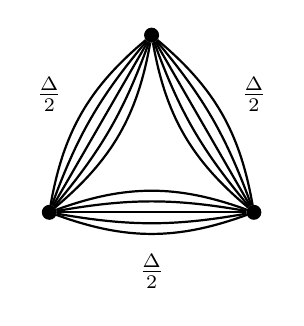
\begin{tikzpicture}[scale=1.5,
            vertex/.style={circle, draw, minimum size=5pt, fill=black, inner sep=0pt},
            edge/.style={thick}
        ]

        % Define positions for the 3 vertices arranged in a triangle
        \foreach \i [count=\n from 1] in {90, 210, 330} {
                \node[vertex] (v\n) at (\i:1) {};
            }

        % Connect each vertex to its two neighbors with multiple edges
        \foreach \n in {1,...,3} {
                % Calculate the next index modulo 3
                \pgfmathtruncatemacro{\next}{mod(\n,3)+1}

                % Draw two parallel edges to represent multiple connections
                \foreach \angle in {-20, -10, ..., 20} {
                        \draw[edge] (v\n) to[bend left=\angle] (v\next);
                    }
                
                \pgfmathtruncatemacro{\angle}{mod(\n+1,3)*120+30}
                \node at (\angle:1) {\(\frac{\Delta}{2}\)};
            }
    \end{tikzpicture}
    \caption{A class of multigraphs with \(\Delta(G)\) even and \(\chi'(G) = \frac{3\Delta(G)}{2}\).}
    \label{fig:vizing-multigraph-counterexample}
\end{figure}

\begin{theorem}[Sharron] \label{thm:sharron}
    Let \(G\) be a multigraph without loops.
    Then,
    \begin{equation}
        \chi'(G) \leq \left\lceil \frac{3\Delta(G)}{2} \right\rceil.
    \end{equation}
\end{theorem}

The class of graphs in Figure~\ref{fig:vizing-multigraph-counterexample} shows that the bound in Theorem~\ref{thm:sharron} is tight (at least for even \(\Delta(G)\)).

\begin{theorem} \label{thm:bipartite-edge-coloring}
    Let \(G\) be a bipartite multigraph without loops.
    Then, \(\chi'(G) \leq \Delta(G)\).
\end{theorem}

\begin{proof}
    If \(\Delta(G)\) is zero, then \(G\) is empty and the result is true.

    Assume that \(\Delta(G) \geq 1\).
    Assume, by induction, that the theorem holds for all bipartite multigraphs with maximum degree at most \(\Delta(G) - 1\).
    Without loss of generality, assume that \(G\) is \(\Delta\)-regular.
    By Hall's Theorem, there exists a perfect matching \(M_\Delta\) in \(G\).
    Let \(G' = G - M_\Delta\).
    Then, \(G'\) is \((\Delta-1)\)-regular.
    By induction, there exists an edge coloring of \(G'\) with \(\Delta-1\) colors.
    Since \(M_\Delta\) is a perfect matching, we can color the edges in \(M_\Delta\) with a new color.
    Therefore, we have an edge coloring of \(G\) with \(\Delta\) colors.
\end{proof}

Let the \vocab{odd girth} of a multigraph \(G\),
denoted \(g_0(G)\),
be the length of the shortest odd cycle in \(G\).
If \(G\) is bipartite, then \(g_0(G) = \infty\).

\begin{theorem}[Goldberg] \label{thm:goldberg}
    Let \(G\) be a multigraph without loops.
    Then,
    \begin{equation}
        \chi'(G) \leq \Delta(G) + 1 + \left\lfloor \frac{\Delta(G) - 2}{g_0(G) - 1} \right\rfloor.
    \end{equation}
\end{theorem}

Note that Theorem~\ref{thm:sharron} is a colorary of Theorem~\ref{thm:goldberg} by using the fact that \(g_0(G) \geq 3\).

Let \(G\) be a multigraph and \(f\) be a edge coloring of \(G - e_0\).
Denote by \(|f|\) the number of colors used in \(f\).
We say that a path \(P = v_0e_0v_1e_1v_2\cdots e_{k-1}v_k\) is a \vocab{valid path with respect to \(f\)} if
\begin{itemize}
    \item \(e_0\) is the uncolored edge,
    \item for every \(i \geq 0\), \(v_i\) is missing some color in \(\{1, 2, \ldots, |f|\}\),
    \item for every \(i \geq 1\), there exists some \(j < i\) such that \(f(e_i)\) is missing at \(v_j\).
\end{itemize}

\begin{lemma}[Kierstead] \label{lem:kierstead}
    Let \(f\) be an edge coloring of a multigraph \(G - e_0\).
    Suppose \(P\) is a valid path with respect to \(f\)
    such that some color \(r\) is missing at two distinct vertices
    \(v_i\) and \(v_j\) in \(P\).
    Then, \(G\) has an edge coloring with \(|f|\) colors.
\end{lemma}

\begin{proof}
    We may assume that \(j < i\).
    The proof is by induction, first on \(i\), then on \(i-j\).

    If \(i = 1\), then \(j = 0\) and therefore we can color \(e_0\) with color \(r\) to get an edge coloring of \(G\) with \(|f|\) colors.

    If \(i-j = 1\), then \(v_j = v_{i-1}\) and we recolor \(e_{i-1}\) with color \(r\)
    to obtain a coloring \(f'\).
    Let \(b = f(e_{i-1})\).
    We know that, in \(f\), \(b\) is missing on \(v_k\) for some \(k < i-1\).
    In \(f'\), \(b\) is missing at \(v_{i-1}\).
    Now, \(v_0e_0v_1e_1\cdots e_{i-2}v_{i-1}\) is a valid path with respect to \(f'\),
    and hence by induction (with a smaller \(i\)), \(G\) has an edge coloring with \(|f|\) colors.

        Assume \(i \geq 2\) and \(i-j \geq 2\).
    We may assume that the colors missing on \(v_1, v_2, \ldots, v_{i-1}\) are distinct.

    Let \(b\) be a color missing at \(v_{i-1}\) in \(f\).
    Let \(Q\) be a maximum \((r, b)\)-alternating path starting at \(v_{j+1}\).
    Note that \(Q\) cannot end at a vertex \(v_k\) with \(k < j\).

    Assume \(Q\) does not end at \(v_j\).
    Obtain \(f'\) from \(f\) by swapping \(r\) and \(b\) on \(Q\).
    Now, \(v_0e_0v_1e_1\cdots v_je_jv_{j+1}\) is a valid path with respect to \(f'\),
    and hence by induction (with a smaller \(i\)), \(G\) has an edge coloring with \(|f|\) colors.

    Assume \(Q\) ends at \(v_j\).
    Obtain \(f'\) from \(f\) by swapping \(r\) and \(b\) on \(Q\).
    Now, \(P\) is valid with respect to \(f'\),
    and hence by induction (with a smaller \(i-j\)), \(G\) has an edge coloring with \(|f|\) colors.
\end{proof}

\begin{proof}[Proof of Theorem~\ref{thm:goldberg}]
    Assume, for the sake of contradiction, that \(G\) is the graph with the smallest number of edges for which the theorem is false.
    Hence,
    \begin{equation}
        \chi'(G) > \Delta(G) + 1 + \frac{\Delta(G) - 2}{g_0(G) - 1}
    \end{equation}
    and \(G - e_0\) has is \((\chi'(G) - 1)\)-edge-colorable,
    where \(e_0\) is an edge of \(G\) with endpoints \(v_0\) and \(v_1\).

    Let \(f\) be an edge coloring of \(G - e_0\) with \(|f| = \chi'(G) - 1\) colors.
    Since \(\chi'(G) - 1 > \Delta(G)\),
    at least \(\chi'(G) - 1 - \Delta(G)\) colors are missing at each vertex of \(G - e_0\) in \(f\).

    Let \(Q\) be a maximum \((r, b)\)-alternating path in \(G - e_0\) starting at \(v_1\).

    Assume \(Q\) does not end at \(v_0\).
    Let \(f'\) be the edge coloring obtained from \(f\) by swapping \(r\) and \(b\) on \(Q\),
    and coloring \(e_0\) with color \(r\).
    Then, \(f'\) is an edge coloring of \(G\) with \(\chi'(G) - 1\) colors, a contradiction.

    Otherwise, assume \(Q\) ends at \(v_0\).
    Therefore, \(Q + e_0\) is an odd cycle of length \(\ell \geq g_0(G)\).
    If the color missing at the vertices of \(Q\) are not distict,
    then by Lemma~\ref{lem:kierstead},
    \(G\) has an edge coloring with \(\chi'(G) - 1\) colors, a contradiction.
    Assume that the colors missing at the vertices of \(Q\) are distinct.
    Therefore, since the number of colors missing at each vertex \(v\) of \(Q\) is at least \(\chi'(G) - 1 - \deg_G(v)\)
    and these colors are distinct,
    the total number of colors missing at the vertices of \(Q\) is at least
    \begin{equation}
        (\chi'(G) - 1 - \Delta(G)) \ell + 2.
    \end{equation}
    Therefore, we can bound the total number of colors in \(G - e_0\) by
    \begin{equation}
        \chi'(G) - 1 \geq (\chi'(G) - 1 - \Delta(G)) g_0(G) + 2,
    \end{equation}
    and hence, by rearranging terms,
    \begin{equation}
        \chi'(G) \leq \Delta(G) + 1 + \frac{\Delta(G) - 2}{g_0(G) - 1},
    \end{equation}
    a contradiction.
\end{proof}

\section{List coloring}

A \vocab{list assignment} of a graph \(G\) is a function
\(L \colon V(G) \to 2^{\{1, 2, \ldots\}}\),
that assigns to each vertex \(v\) a set \(L(v)\) of colors (commonly called the \vocab{list} of \(v\)).
An \vocab{\(L\)-list-coloring} of \(G\) is a function
\(c \colon V(G) \to \{1, 2, \ldots\}\)
such that \(c(v) \in L(v)\) for all \(v \in V(G)\).

We say that \(G\) is \vocab{\(k\)-list-colorable} if for every list assignment \(L\) of \(G\) with \(|L(v)| \geq k\) for all \(v \in V(G)\),
there exists an \(L\)-list-coloring of \(G\).
We write \(\chi_\ell(G)\) for the minimum \(k\) such that \(G\) is \(k\)-list-colorable.

\begin{proposition}
    Let \(G\) be a graph.
    Then,
    \begin{equation}
        \chi(G) \leq \chi_\ell(G).
    \end{equation}
\end{proposition}

\begin{proof}
    The constant list \(L(v) = \{1, 2, \ldots, \chi(G) - 1\}\) for all \(v \in V(G)\) does not admit an \(L\)-list-coloring of \(G\).
    Hence, \(\chi_\ell(G) > \chi(G) - 1\), and therefore \(\chi(G) \leq \chi_\ell(G)\).
\end{proof}

Hence, an edge coloring of \(G\) is equivalent to a vertex coloring of \(L(G)\).
We define the \vocab{list chromatic index} of a graph \(G\) as \(\chi'_\ell(G) = \chi_\ell(L(G))\), where \(L(G)\) is the line graph of \(G\).

\begin{proposition}
    Let \(G\) be a graph.
    Then,
    \begin{equation}
        \chi'_\ell(G) \leq 2 \Delta(G) - 1.
    \end{equation}
\end{proposition}

\begin{theorem}[Behzad--Vizing's Conjecture (1975)]
    \label{thm:behzad-vizing-conjecture}
    Let \(G\) be a graph.
    Then,
    \begin{equation}
        \chi'_\ell(G) = \chi'(G).
    \end{equation}
\end{theorem}

\begin{theorem}[Dinitz's Conjecture (1979), Galvin's Theorem (1995)]
    \label{thm:dinitz-galvin}
    \begin{equation}
        \chi'_\ell(K_{n, n}) = \chi'_\ell(K_{n, n}) = n.
    \end{equation}
\end{theorem}

We show the proof of Theorem~\ref{thm:dinitz-galvin}.

\begin{definition}[Kernel]
    A \vocab{kernel} in a directed graph \(D\) is
    a subset \(K \subseteq V(D)\) that is
    independent and
    absorbing, i.e.,
    for each \(v \in V(D) \setminus K\),
    there exists \(u \in K\) such that
    \(D\) has an arc from \(v\) to \(u\).
\end{definition}

\begin{lemma}[Bondy--Boppana--Segal] \label{lem:bondy-boppana-segal}
    Let \(D\) be a directed graph such that
    every induced subgraph of \(D\) has a kernel.
    Then, \(D\) has an \(L\)-list-coloring
    for any list assignment \(L\)
    such that, for each \(v \in V(D)\),
    \begin{equation}
        |L(v)| \geq \deg^+(v) + 1,
    \end{equation}
    where \(\deg^+(v)\) denotes the out-degree of \(v\).
\end{lemma}

\begin{proof}
    We proceed by induction on \(|V(D)|\).
    Assume,
    as the induction hypothesis,
    that the lemma holds for all directed graphs with fewer vertices than \(D\).
    If \(|V(D)| \leq 1\), then the lemma is trivially true.

    Assume that \(|V(D)| \geq 2\).
    Let \(\alpha \in \bigcup_{v \in V(D)} L(v)\).
    Let \(D_0\) be the subgraph of \(D\) induced by \(\{v \in V(D) : \alpha \in L(v)\}\),
    which is non-empty.
    Since \(D_0\) is an induced subgraph of \(D\), \(D_0\) has a kernel \(K\), which is also non-empty.
    Let \(D'\) be the subgraph of \(D\) induced by \(V(D) \setminus K\).
    Define the list assignment \(L'\) on \(D'\) by
    \begin{equation}
        L'(v) = \begin{cases}
            L(v) & \text{if } v \notin V(D_0), \\
            L(v) \setminus \{\alpha\} & \text{if } v \in V(D_0).
        \end{cases}
    \end{equation}
    Then, for each \(v \in V(D')\),
    \begin{equation}
        |L'(v)| \geq \deg^+_{D'}(v) + 1,
    \end{equation}
    since any \(v\) with \(\alpha \in L(v)\) has an arc to \(K\) in \(D\).

    Finally, by the induction hypothesis,
    \(D'\) has an \(L'\)-list-coloring \(c'\).
    Since \(K\) is independent,
    the coloring \(c\) obtained from \(c'\)
    by assigning \(\alpha\) to each vertex in \(K\)
    is an \(L\)-list-coloring of \(D\), as required.
\end{proof}

\begin{theorem}[Galvin's Theorem (1995)] \label{thm:galvin}
    For any bipartite graph \(G\),
    \begin{equation}
        \chi'_\ell(G) = \chi'(G) = \Delta(G).
    \end{equation}
\end{theorem}

\begin{proof}
    Let \(G\) be a bipartite graph with vertex classes \(X\) and \(Y\).
    Let \(c\) be an edge coloring of \(G\) with colors \(\{1, 2, \ldots, \Delta(G)\}\).
    We define an orientation \(D\) of \(L(G)\) as follows:
    if \(e\) and \(f\) meet in \(X\),
    then we direct the arc \(e \to f\) where \(c(e) > c(f)\);
    if \(e\) and \(f\) meet in \(Y\),
    then we direct the arc \(e \to f\) where \(c(e) < c(f)\).

    First, note that, for each \(e \in E(G)\),
    we have
    \begin{equation}
        \deg^+_D(e) \leq \Delta(G) - 1,
    \end{equation}
    since \(e\) is the source of at most one arc to a vertex of a given other color.

    We claim that every induced subgraph \(D'\) of \(D\) has a kernel.
    Assume, as the induction hypothesis,
    that the claim holds for all induced subgraphs of \(D\)
    with fewer vertices than \(D'\).
    If \(|V(D')| = 0\), then the empty set is a kernel.
    Assume \(|V(D')| \geq 1\).
    Let
    \begin{equation}
        X' = \{x \in X : x \text{ is a endpoint of an vertex of } D'\}
    \end{equation}
    and let
    \begin{equation}
        U = \left\{
            e_x \in V(D')
            :
            \begin{array}{c}
                x \in X' \text{ and }
                e_x \text{ is the edge in } D' \\
                \text{ incident to } x \text{ of smallest color}
            \end{array}
        \right\}
    \end{equation}
    which is absorbing.
    If \(U\) is independent (i.e., a matching), then \(U\) is a kernel of \(D'\), as desired.
    Otherwise, there exists edges \(e\) and \(f\) in \(U\) that meet in \(Y\).
    Assume that \(c(e) < c(e')\).
    Let \(D'' = D' - \{e\}\).
    By the induction hypothesis, \(D''\) has a kernel \(U'\).
    If \(e' \in U'\), then \(U'\) is a kernel of \(D'\) as well, as desired.
    Otherwise, if \(e' \notin U'\),
    then there exists \(e'' \in U'\) such that \(e' \to e''\).
    By minimality of the color of \(e'\), \(e'\) and \(e''\) cannot meet in \(X\);
    hence, the three edges \(e\), \(e'\), and \(e''\) meet in \(Y\), and \(c(e) < c(e') < c(e'')\), and hence \(e \to e''\), and hence \(U'\) is a kernel of \(D'\), as desired.
\end{proof}

\section{Total coloring}

A \vocab{total coloring} of a graph \(G\) is a function
\(c \colon V(G) \cup E(G) \to \{1, 2, \ldots\}\)
such that no two adjacent or incident elements have the same color.
The smallest number of colors
needed for a total coloring of \(G\)
is denoted by \(\chi''(G)\).

\begin{proposition}
    Let \(G\) be a graph.
    Then,
    \begin{equation}
        \chi''(G) \geq \Delta(G) + 1.
    \end{equation}
\end{proposition}

\begin{proposition} \label{prop:chi''-complete}
    Let \(n\) be a positive integer.
    Then,
    \begin{equation}
        \chi''(K_n)
        =
        \begin{cases}
            \Delta(K_n) + 1 = n & \text{if } n \text{ is odd}, \\
            \Delta(K_n) + 2 = n + 1 & \text{if } n \text{ is even}.
        \end{cases}
    \end{equation}
\end{proposition}

\begin{proposition} \label{prop:chi''-cycle}
    Let \(n\) be a positive integer.
    Then,
    \begin{equation}
        \chi(C_n) =
        \begin{cases}
            3 & \text{if } n \text{ is multiple of } 3, \\
            4 & \text{otherwise}.
        \end{cases}
    \end{equation}
\end{proposition}

\begin{proposition}
    Let \(G\) be a graph.
    Then,
    \begin{equation}
        \chi''(G) \leq 2\Delta(G) + 1.
    \end{equation}
\end{proposition}

\begin{proof}
    If \(G\) is complete or a cycle, then the proposition is true by Propositions~\ref{prop:chi''-complete} and~\ref{prop:chi''-cycle}.
    Assume that \(G\) is not complete or a cycle.
    Moreover, assume that \(G\) is connected.
    \nameref{thm:brooks-theorem} implies that \(\chi(G) \leq \Delta(G)\),
    that is, there exists a vertex coloring of \(G\) with \(\Delta(G)\) colors.
    \nameref{thm:vizing} implies that \(\chi'(G) \leq \Delta(G) + 1\),
    that is, there exists an edge coloring of \(G\) with \(\Delta(G) + 1\) colors.
    The coloring of \(V(G) \cup E(G)\) obtained by disjointly using the vertex and edge colors is a total coloring of \(G\) with \(\Delta(G) + 1 + \Delta(G) = 2\Delta(G) + 1\) colors, as desired.
\end{proof}

\begin{conjecture}[Vizing, 1964]
    Let \(G\) be a graph.
    Then,
    \begin{equation}
        \chi''(G) \leq \Delta(G) + 2.
    \end{equation}
\end{conjecture}

\begin{lemma}
    Let \(G\) be a graph.
    Then,
    \begin{equation}
        \chi''(G) \leq \chi'_\ell(G) + 2.
    \end{equation}
\end{lemma}

\begin{proof}
    Let \(c\) be a vertex coloring of \(G\) with colors \(\{1, 2, \dots, \chi'_\ell(G)+2\}\),
    which is possible since \(\chi'_\ell(G) \geq \Delta(G)\).
    To each edge \(e = xy\), assign the list
    \begin{equation}
        L(e) = \{1, 2, \dots, \chi'_\ell(G) + 2\} \setminus \{c(x), c(y)\}.
    \end{equation}
    Since each list has size \(\chi'_\ell(G)\), by definition,
    there exists an edge coloring \(c'\) that respects this list assignment.
    By uniting the colorings \(c\) and \(c'\), we get a total coloring of \(G\), with \(\chi'_\ell(G)\) colors.
\end{proof}

\begin{theorem}[McDiairmid--Reed] \label{thm:mcdiairmid-reed}
    Let \(G\) be a graph.
    Then,
    \begin{equation}
        \chi''(G) \leq \chi'(G) + t + 1,
    \end{equation}
    where \(t\) is such that \(t! > |V(G)|\).
\end{theorem}

The following proof of Theorem~\ref{thm:mcdiairmid-reed} is probabilistic, not constructive.

\begin{proof}
    Assume \(G\) not complete, and not an odd cycle, otherwise the theorem can be verified directly.
    Let \(\phi\) be an edge coloring of \(G\) using \(\chi'(G)\) colors,
    and let \(f\) be a vertex coloring of \(G\) using \(\chi'(G)\) colors,
    which exists since \(\chi'(G) \geq \Delta(G) \geq \chi(G)\)
    by Proposition~\ref{prop:easy-bounds-edge-coloring}
    and \nameref{thm:brooks-theorem}.
    
    Consider all sets \(A\) of \(t\) edges in \(G\) that are incident to a same vertex and such that the colors assigned to their other endpoints by \(f\) are pairwise distinct.
    Specifically, for each such set \(A = \{e_1, e_2, \ldots, e_t\}\), where \(e_i = v a_i\), we require that \(f(a_i) \neq f(a_j)\) for all \(i \neq j\).
    
    For a permutation \(\pi\) of the colorset \(\{1, 2, \ldots, \chi'(G)\}\), define \(A\) to be \emph{\(\pi\)-bad} if \(\pi(\phi(e_i)) = f(a_i)\) for every \(e_i \in A\).
    
    For any fixed set \(A\), the number of permutations \(\pi\) for which \(A\) is \(\pi\)-bad is \((\chi'(G) - t)!\),
    since the permutation must map each \(\phi(e_i)\) to \(f(a_i)\),
    leaving the remaining \(\chi'(G) - t\) colors to be permuted freely.
    
    The total number of such sets \(A\) is at most \( |V(G)| \binom{\Delta(G)}{t} \),
    as there are at most \(|V(G)|\) choices for the vertex to which the edges in \(A\) are incident,
    and \(\binom{\Delta(G)}{t}\) ways to select \(t\) incident edges from a vertex with maximum degree \(\Delta(G)\).
    
    By the union bound,
    the number of permutations \(\pi\) that render at least one set \(A\) \(\pi\)-bad is at most
    \begin{equation}
        |V(G)| \binom{\Delta(G)}{t} (\chi'(G) - t)!.
    \end{equation}
    
    Since \(t! > |V(G)|\), and \(\chi'(G) \in \{\Delta(G), \Delta(G) + 1\}\) by \nameref{thm:vizing}, we have that
    \begin{itemize}
        \item If \(\chi'(G) = \Delta(G)\), then
        \begin{equation}
            |V(G)| \binom{\Delta(G)}{t} (\chi'(G) - t)!
            = \frac{|V(G)|}{t!} \Delta(G)!
            < \Delta(G)! = \chi'(G)!;
        \end{equation}
        \item and if \(\chi'(G) = \Delta(G) + 1\), then
        \begin{equation}
            |V(G)| \binom{\Delta(G)}{t} (\chi'(G) - t)!
            = \frac{|V(G)|}{t!} \Delta(G)! (\Delta(G) + 1 - t)
            < (\Delta(G) + 1)!  = \chi'(G)!.
        \end{equation}
    \end{itemize}
    
    Therefore,
    in both cases,
    the total number of permutations \(\pi\) that render at least one set \(A\) \(\pi\)-bad is strictly less than \(\chi'(G)!\),
    implying that there exists a permutation \(\sigma\) such that no set \(A\) is \(\sigma\)-bad.
    
    Define the subgraph \(H\) of \(G\) to consist of edges \(xy\) where \(\sigma(\phi(xy)) \in \{ f(x), f(y) \}\).
    Since no set \(A\) is \(\sigma\)-bad, each vertex is incident to at most \(t\) edges in \(H\), ensuring that \(\Delta(H) \leq t\).
    By \nameref{thm:vizing}, \(H\) can be edge-colored with \(t + 1\) colors, say using a coloring \(\psi\) with colorset \(\{\chi'(G) + 1, \chi'(G) + 2, \ldots, \chi'(G) + t + 1\}\).
    
    Finally, define the total coloring \(c\) of \(G\) by
    \begin{align}
        c(v) & = f(v)            && \text{for all } v \in V(G),                \\
        c(e) & = \sigma(\phi(e)) && \text{for all } e \in E(G) \setminus E(H), \\
        c(e) & = \psi(e)         && \text{for all } e \in E(H).
    \end{align}
    This is a proper total coloring of \(G\) using \(\chi'(G) + t + 1\) colors, as desired.
\end{proof}

We remark that this proof can be optimized to show that \(\chi''(G) \leq \chi'(G) + t\).